\section{Measurements and evaluation}\label{measurements-and-evaluation}

\subsection{Measurement of relaxation time}\label{relaxation-time}

We measure $T_1$ and $T_2$ once with the spin echo method and $T_2$ again with the Carr-Purcell sequence for each Gd 500 and Gd 600.
\begin{table}[h!]
\centering
\begin{tabular}{c||c|c|c}
probe  &  $T_{1,SE}$ & $T_{2,CP}$ & $T_{2,SE}$ \\
\hline
\hline
Gd 500 & 68.1 & 66.1 & 62.4 \\
\hline
Gd 600 & 99.2 & 84.0 & 78.6 \\
\end{tabular}
\caption{Summary of relaxation time measurements in $ms$}
\label{table1}
\end{table}\\
We can see 3 relations from these measurements: $T_{1} > T_{2}$ and $T_{2,CP} > T_{2,SE}$ for both substances as well as $T_{600} > T_{500}$ for each different method.\\
The first can be explained by that $T_2$ contains additionally the effects of interactions of an ensemble of spins dephasing from each other.\\
The second relation can be explained by looking at the effects of the Carr-Purcell method. This method minimizes the effects of the molecular diffusion and field inhomogeneities, which improves the precision of greater echo times.\\
The third relation can be attributed to the fact that the Gd 500 has higher concentration of Gd. The excitation energy of protons is dissipated in another way by interacting with Gd spins. Thus the more Gd there is, the shorter is the relaxation time.\\
From $\omega_L = 2\pi\cdot19.8 MHz  $ we can calculate our external field $\vec{B_0}$. And with the characteristic time $\Delta t = 1.29\cdot 10^{-6}s $ for a $90\degree$ pulse we can calculate the solenoidal field $\vec{B_1}$ as well.
\begin{equation}
	B_0 = \dfrac{\omega_L}{\gamma} = 0.48 T
\end{equation}
\begin{equation}
	B_1 = \dfrac{\alpha}{\Delta t \gamma} = 4.3 mT
\end{equation}
with $\gamma$ being the gyromagnetic factor mentioned in section \ref{basics}.\\
\subsection{Chemical shift}\label{chemical-shift}

We measure the peaks and determine which peak is the TMS. After that we calculate the shift with the ppm, which is short for parts per million, given by the .vi and appoint them to a substance from figure \ref{shi2} with the help of the provided reference sheet seen in figure \ref{shi1}. The ppm to calculate the difference was read out of the .vi like in figure \ref{Lab2}. \\
\begin{table}[h!]
\centering
\begin{tabular}{c||c|c|c|c|c}
 & A+ & B+ & C+ & D+ & E+ \\
\hline
\hline
$\Delta$(2nd - TMS) & 2.2 & 2.1 & 2.0 & 3.9 & 2.6 \\
\hline
$\Delta$(3rd - TMS) & 3.9 & 6.9 & 11.6 & 6.3 & 7.5 \\
\hline
$\Delta$(4th - TMS) & 6.3 &  &  &  & \\
\hline
\hline
Substance & fluoroacetone & p-xylol & acetic acid & fluoroacetonitril & toluol \\
\end{tabular}
\caption{Summery of chemical shift in ppm}
\label{table2}
\end{table}\\
Even though the resonance frequency of Flour is much higher than the frequency we are using here, we can see the peaks caused by the Flour. They appear because of the spin-spin interaction between Flour and the proton (hydrogen) in FCH$_2$, which leads to 2 different states for the electrons. For both D+ and A+ we can see each of these peaks at 3.9 and 6.3 on both spectra.
\vspace{2mm}\\
From the width of these peaks we can additionally calculate the energy resolution of this measurement as well, as the energy difference between the 2 different states FCH$_2$ can be in, depending on the spin-spin interaction of the electrons.
\begin{equation}\label{E_r}
	\Delta E_{res} = f_{FWHM} \cdot h = 19.9 Hz \cdot 4.136eVs = 8 \cdot 10^{-14}eV
\end{equation}
\begin{equation}\label{E_d}
	\Delta E_{dipole} = f_{\Delta F} \cdot h = 48 Hz \cdot 4.136eVs = 2 \cdot 10^{-13}eV
\end{equation}\\
\subsection{Imaging with NMR}\label{imaging-with-nmr}
\begin{figure}[h]
	\begin{subfigure}{0.32\textwidth}
	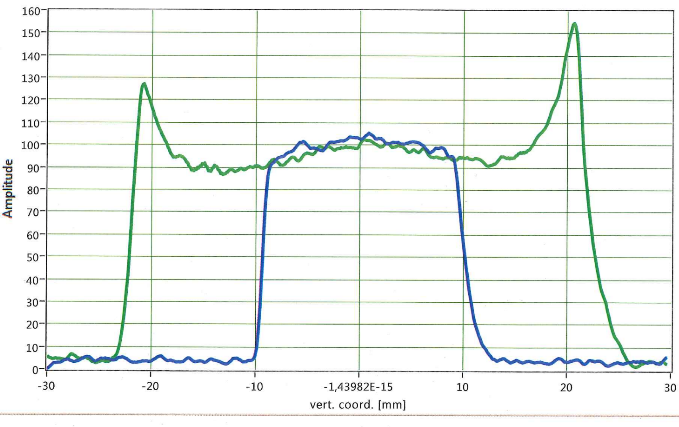
\includegraphics[width=0.9\linewidth ,height=4cm]{images/oil15_50.png}
	\caption{15 mL and 50 mL Oil}
	\label{NMR1}
	\end{subfigure}
	\begin{subfigure}{0.32\textwidth}
	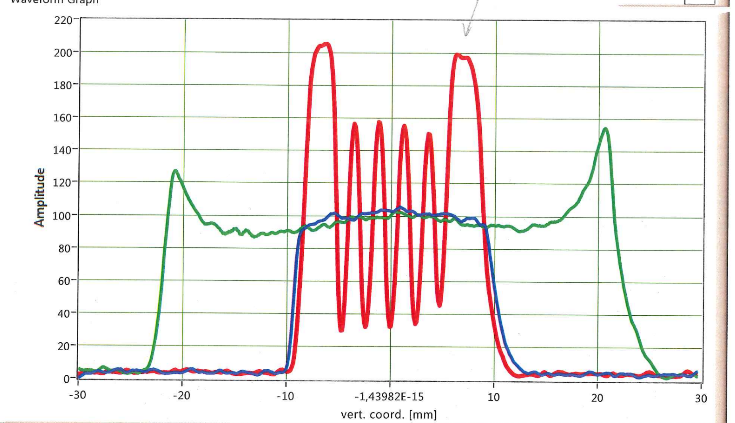
\includegraphics[width=0.9\linewidth ,height=4cm]{images/oil_teflon.png}
	\caption{Oil and Teflon (red graph)}
	\label{NMR2}
	\end{subfigure}
	\begin{subfigure}{0.32\textwidth}
	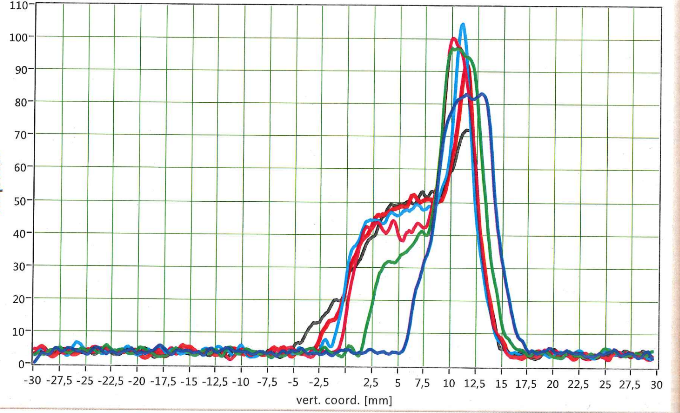
\includegraphics[width=0.9\linewidth, height=4cm]{images/oil_sand.png}
	\caption{Oil on Sand over time}
	\label{NMR3}
	\end{subfigure}
	\caption{NMR imaging 1D}
\end{figure}
First we set the analyser in 1D mode. We poured 15 mL oil in a tube and could observe the capillary effect of the liquid on the glass of the tube. Then we added 35 mL oil, in total 50 mL, in the tube and we could see the boundaries of the analyser. They are caused by the inhomogeneity of the magnetic field when probes are placed too far from the center of the coils. Both measurements can be seen in figure \ref{NMR1}. \\
Then we put a teflon slice inside the oil tube and kept it partly immersed in oil. Dips on figure \ref{NMR2} show us that the Teflon layers aren't NMR-active.\\
Subsequently we filled an empty tube with 15 mm sand and 4 mm oil on top of it. We observed it in the analyser while the oil was seeping through the sand as shown in figure \ref{NMR3}. Though one might think that seeping of oil into sand could be compared to the diffusion of gas, the figure shows it is not the case, since it has seemingly random plateaus and drops in the seeping process. \\
For the 2D imaging we inserted various objects into the analyser and displayed them with a LabView .vi. In figure \ref{2DNMR} are some of the images we made. \\
\begin{figure}[h]
	\begin{subfigure}{0.32\textwidth}
	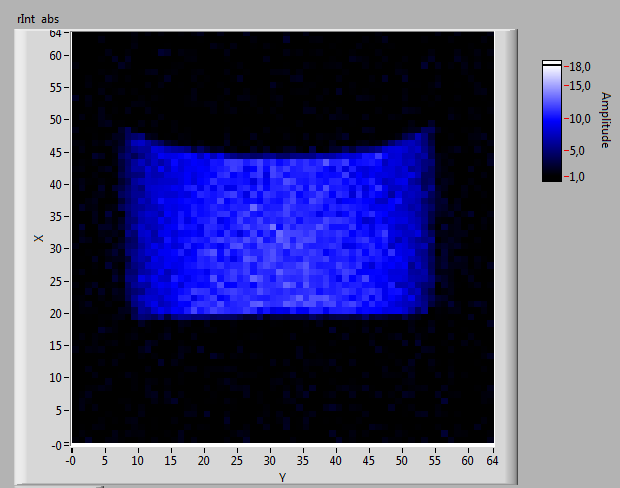
\includegraphics[width=0.9\linewidth ,height=4cm]{2d_image/Oil_Vertical_15_2.png}
	\caption{15 ml Oil 2D}
	\label{2DNMR1}
	\end{subfigure}
	\begin{subfigure}{0.32\textwidth}
	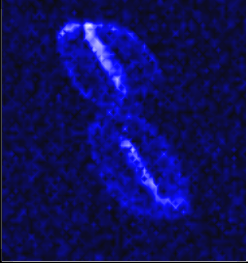
\includegraphics[width=0.9\linewidth ,height=4cm]{2d_image/peanut_5avg_2_3d.png}
	\caption{Peanuts in Shell}
	\label{2DNMR2}
	\end{subfigure}
	\begin{subfigure}{0.32\textwidth}
	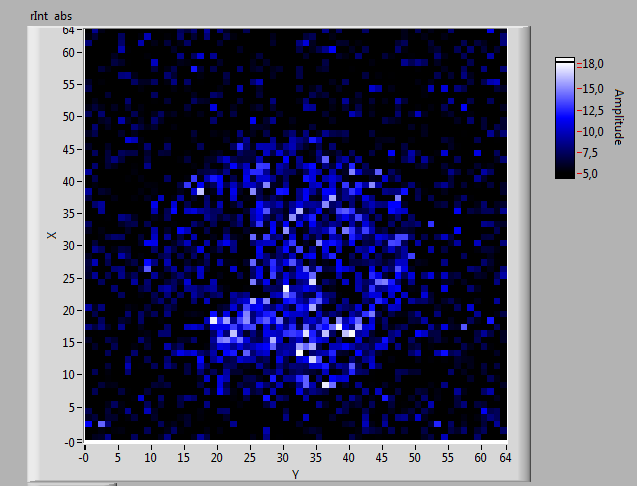
\includegraphics[width=0.9\linewidth, height=4cm]{2d_image/tomato_2.png}
	\caption{A Cherry Tomato}
	\label{2DNMR3}
	\end{subfigure}
	\caption{NMR imaging 2D}
	\label{2DNMR}
\end{figure} \\
Figure \ref{2DNMR1} is the 15 mL oil tube used for figure \ref{NMR1} being imaged in 2D. One can still see the capillary effect on the edges of the tube. \\
In figure \ref{2DNMR2} a peanut is imaged. The white stripes between the two halves of a single nut is the air between the two halves. All of this can be observed without even opening the shell, which illustrates the power of this technique. \\
Finally we took a picture of horizontal slice of a cherry tomato, as shown in figure \ref{2DNMR3}. Since the cherry tomato contains and is mainly consists of water, which is not NMR-active, it's difficult to differentiate the signal of object itself and its surrounding noise, and hence the image only shows a blurry shape.\\